% 原文 pp.188--194
% 原文 p.188
\hypertarget{srcpage:188}{}\label{srcpage:188}
\subsubsectionlink{Ohmicなデコヒーレンスと散逸}
中心系が調和振動子である量子Brown運動のマスター方程式(5.25)に現れる係数$\widetilde\Omega^2$、$\gamma$、$D$、$f$［(5.26)参照］を、さらに評価しよう。そのためには、$\nu(\tau)$、$\eta(\tau)$の表式［(5.16)、(5.17)参照］に入るスペクトル密度$J(\omega)$の、具体的な関数形を選ばなければならない。

前述のように、通常は、$J(\omega)$の元の表式(5.18)の離散的な和を、しばしば現象論的に動機づけられた、環境振動数$\omega$の連続関数に置き換える。一般に、$J(\omega)$の振動数依存性は、$J(\omega)\propto\omega^\alpha$というべき則に従うとする。指数$\alpha$の最も普通の選択は$\alpha=1$、すなわち$J(\omega)$が$\omega$とともに線形に増える場合である。この種類のスペクトル密度はOhmicと呼ばれる（名称は、スピン・ボソン模型の散逸効果の解析に由来する）。他の、より重要性の低い例として、$\alpha<1$のsubohmicなスペクトル密度と、$\alpha>1$のsupraohmicなスペクトル密度がある。

ここでは、Ohmicなスペクトル密度$J(\omega)\propto\omega$の場合に注目し、具体的に
\chfiveeq{43}
と書こう。定数$\gamma_0$は、系と環境の実効的な結合強度を記述する。スペクトル密度の元の離散的表式(5.18)では、この相互作用強度は、個々の振動子結合$c_i$を含む項の和で表されていた。まもなく見るように、$\gamma_0$は振動数に依存しない減衰定数として働く（具体的な実験状況に基づく現象論的なデコヒーレンス模型では、しばしば$\gamma_0$を測定データから導く）。

$J(\omega)$の振動数依存性がべき則ならば、環境の振動数分布は際限なく増大することになる。しかし、これは物理的に妥当ではない。通常、$J(\omega)$の$\omega$に対する線形依存性は、小さい$\omega$でしか成り立たず、高振動数へ向かって弱まる。そのため、普通は高振動数カットオフ$\Lambda$を選び、$\omega>\Lambda$の振動数で$J(\omega)$を減衰させる項を含めるように、(5.43)を修正する。よく用いられるのは、いわゆるLorentz--Drude形のカットオフ項である。
\chfiveeq{44}
このスペクトル密度のグラフを図5.2に示す。意図したとおり、カットオフ$\Lambda$を超える環境振動数$\omega$では、対応する振動数密度$J(\omega)$が減少する。

スペクトル密度$J(\omega)$の具体的選択(5.44)により、係数$\widetilde\Omega^2$、$\gamma$、$D$、$f$［(5.26)参照］を計算できるようになる。

% 原文 p.189
\hypertarget{srcpage:189}{}\label{srcpage:189}
\begin{figure}[htbp]\centering
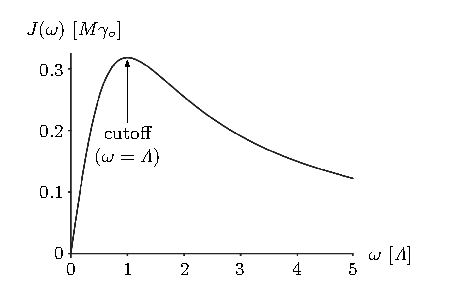
\includegraphics[width=.65\linewidth]{figures/ch05_fig02.pdf}
\caption{(5.44)のスペクトル密度$J(\omega)$のグラフ（単位：$M\gamma_0$）。$J(\omega)$は、高振動数カットオフ$\Lambda$より十分低い振動数$\omega$ではほぼ線形に増加し、その後$\omega>\Lambda$では減少する。振動数軸の単位はカットオフ$\Lambda$である。}\label{fig:5.2}
\end{figure}
運動量減衰係数$\gamma$と通常拡散係数$D$は、特に容易に評価できる。これを見るため、雑音核$\nu(\tau)$［(5.16)参照］は、前の因子$\sqrt{2/\pi}$がないことを除けば、関数$J(\omega)\coth(\omega/2k_{\mathrm B}T)$のFourier余弦変換にすぎないことに注意しよう。同様に、散逸核$\eta(\tau)$［(5.17)参照］は、$J(\omega)$のFourier正弦変換に比例する。さらに、$\gamma$の表式［(5.26b)参照］を見ると、これは$\eta(\tau)$のFourier正弦変換に比例している。

ところが、奇関数$g(-x)=-g(x)$に対して、2回のFourier正弦変換は元の関数を与える。
\chfiveeq{45}
スペクトル密度(5.44)は$\omega$の奇関数であり、$\gamma$は、前の因子を除けば$J(\omega)$を2回Fourier正弦変換したものなので、$\gamma$は、系の調和振動子の振動数$\Omega$で評価した$J(\omega)$に単純に比例する［(5.26b)、(5.45)と比較］。2回のFourier変換の定義(5.45)から生じる因子$2/\pi$を考慮すると、
\chfiveeq{46}
を得る。マスター方程式(5.25)の運動量減衰係数$\gamma$と、スペクトル密度の表式(5.43)で導入した実効結合強度$\gamma_0$とのこの関係は、$\gamma_0$を振動数に依存しない減衰定数とみなせるという、先の主張を正当化する。スペクトル密度にカットオフを課さなければ（$\Lambda\to\infty$）、$\gamma$と$\gamma_0$は厳密に等しい。

通常拡散係数$D$［(5.26b)参照］の計算も、同様の議論に従う。$D$は、$J(\omega)\coth(\omega/2k_{\mathrm B}T)$を2回Fourier余弦変換したものに比例する。

% 原文 p.190
\hypertarget{srcpage:190}{}\label{srcpage:190}
偶関数$g(-x)=g(x)$に対しては、このような2回のFourier余弦変換について、(5.45)と類似の恒等式
\chfiveeq{47}
が成り立つ。関数$J(\omega)\coth(\omega/2k_{\mathrm B}T)$は、確かに$\omega$について偶関数なので、
\chfiveeq{48}
を得る。$D$の温度依存性を図5.3に示す。$D$は温度とともに増大する。すなわち、環境の温度を上げるほどデコヒーレンスは強くなる。高温$k_{\mathrm B}T\gg\Omega$では、$\coth(\Omega/2k_{\mathrm B}T)\approx2k_{\mathrm B}T/\Omega$なので、$D$は温度にほぼ線形に増大する（この高温極限は後の5.2.4節で詳しく調べる）。

振動数の繰り込み$\widetilde\Omega^2$［(5.26a)参照］の表式は、Fourier正弦変換のFourier余弦変換である。この場合、(5.45)、(5.47)の形の簡単な恒等式はないが、この係数を具体的に評価するのは、かなり容易である。ここでは導出を示さず、結果だけを述べる。
\chfiveeq{49}
最後に、異常拡散係数$f$［(5.26d)参照］は、$\coth(\omega/2k_{\mathrm B}T)$の項があるため、評価がより難しい。比較的容易に扱えるのは、$k_{\mathrm B}T\gg\Omega$となる高温環境の場合である（次節参照）。この極限では、得られる$f$の表式は、通常拡散係数(5.48)に比べて、カットオフ振動数$\Lambda$程度の因子だけ小さい。
\begin{figure}[htbp]\centering
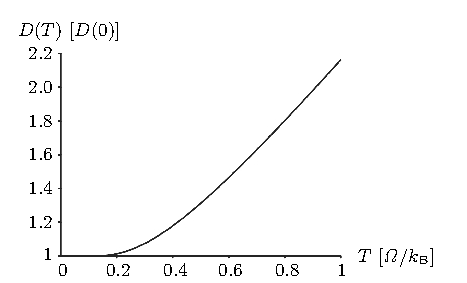
\includegraphics[width=.65\linewidth]{figures/ch05_fig03.pdf}
\caption{Ohmicなスペクトル密度(5.44)の場合の、通常拡散係数$D$［(5.48)参照］の温度依存性。縦軸の単位は、通常拡散係数の零温度値$D(T=0)$、温度軸の単位は$\Omega/k_{\mathrm B}$である。}\label{fig:5.3}
\end{figure}

% 原文 p.191
\hypertarget{srcpage:191}{}\label{srcpage:191}
\subsubsectionlink{Caldeira--Leggettマスター方程式}
以下では、高温環境の極限を詳しく調べよう。すなわち、環境の熱エネルギー$k_{\mathrm B}T$が、系の固有振動数$\Omega$と環境のカットオフ振動数$\Lambda$に対応するエネルギーより、はるかに大きい状況を考える。このとき、通常拡散係数$D$の表式(5.48)に現れる$\coth(\Omega/2k_{\mathrm B}T)$を、$2k_{\mathrm B}T/\Omega$で近似できる。これは、$\Omega/2k_{\mathrm B}T=0$のまわりの$\coth(\Omega/2k_{\mathrm B}T)$のTaylor展開の1次の項である。この場合、係数$D$は
\chfiveeq{50}
となる。また、環境振動数の上限領域であるカットオフ$\Lambda$は、系の特徴的振動数$\Omega$より、はるかに大きいと仮定する。すると(5.50)は
\chfiveeq{51}
という形になる。さらに、運動量減衰係数$\gamma$［(5.46)参照］は、実効結合強度$\gamma_0$の値に近づき、
\chfiveeq{52}
振動数の繰り込み$\widetilde\Omega^2$［(5.49)参照］は
\chfiveeq{53}
となる。最後に、ここで考える仮定のもとでは、異常拡散係数$f$を具体的に評価でき、
\chfiveeq{54}
を得る。

対応する異常拡散項$f[\hat X,[\hat P,\hat\rho_{\mathrm S}(t)]]$がマスター方程式(5.25)でどの程度重要かをさらに知るため、この項と$D[\hat X,[\hat X,\hat\rho_{\mathrm S}(t)]]$の大きさを比較しよう。その大きさは、それぞれ、およそ
\chfiveeq{55}
および
\chfiveeq{56}
である。

% 原文 p.192
\hypertarget{srcpage:192}{}\label{srcpage:192}
仮定により$\Lambda\gg\Omega$なので、ここではマスター方程式(5.25)の異常拡散項を、問題なく無視できる。

係数$D$、$\gamma$、$\widetilde\Omega^2$の上の表式(5.51)、(5.52)、(5.53)を、Born--Markovマスター方程式(5.25)へ代入しよう。結果は
\chfiveeq{57}
となり、系の、振動数をシフトしたHamiltonian $\hat H'_{\mathrm S}$は
\chfiveeq{58}
である。(5.57)の右辺に現れる項の解釈は、マスター方程式の、より一般的な形(5.25)について、すでに論じた（5.2.2節参照）。第1項は、振動数をシフトしたHamiltonianによる、通常のLiouville--von Neumann項である。第2項は、$\gamma_0$に比例する特徴的な率の運動量減衰、すなわち散逸を記述する。第3項は、位置基底のデコヒーレンスと、それに伴う運動量拡散を表し、その温度依存の特徴的な局在化率は、係数$M\gamma_0k_{\mathrm B}T$と、隔たりの二乗$(X-X')^2$の積で与えられる。

方程式(5.57)は、一般にCaldeira--Leggettマスター方程式として知られる（ここでは中心系が調和振動子の場合について書いた）。これは1980年代初頭に、CaldeiraとLeggettが経路積分法を用いて初めて導いた\cite{ref221}。デコヒーレンス過程と散逸過程の模型化に、広く用いられる。実際、導出の基礎となる仮定が厳密には満たされない状況でも、しばしばかなりうまく適用されてきた（例えば、$k_{\mathrm B}T\lesssim\Lambda$となることの多い量子光学の状況\cite{ref222}）。

Caldeira--Leggettマスター方程式の特に魅力的な性質は、デコヒーレンス率と、その率と散逸の関係する率との関係を、非常に直観的かつ簡単に見積もれることである。これを見るため、温度$T$の、質量$M$の粒子の熱的de Broglie波長が、通常どおり$\hbar\equiv1$とすると、［(2.114)参照］
\chfiveeq{59}
で与えられることを思い出そう。したがって位置表示を用いれば、(5.57)の右辺の最終項は
\chfiveeq{60}
と書ける。

% 原文 p.193
\hypertarget{srcpage:193}{}\label{srcpage:193}
この項は、［(3.58)、(5.36)と比較］
\chfiveeq{61}
というデコヒーレンス率$\tau_{|X-X'|}^{-1}$での空間的局在化を記述する。デコヒーレンス率と減衰率$\gamma_0$の比は、空間的隔たりと物体の熱的de Broglie波長(5.59)の比の二乗に等しいことがわかる。定数$\gamma_0^{-1}$は系の散逸（緩和）時間尺度を定量化するので、(5.61)は、2.11節で導出なしに与えた表式(2.113)そのものである。そこで述べたように、量子Brown運動模型から導かれる表式(5.61)は、1980年代初頭に、デコヒーレンス時間尺度という概念を導入するため、Zurekが初めて用いた\cite{ref012}。同じ節で、熱的de Broglie波長は巨視的物体、さらには中間的な大きさの物体でも極端に小さいと指摘した。したがって、巨視的に離れた重心位置の重ね合わせで記述される物体は、通常、緩和時間尺度より何桁も短い時間尺度で、デコヒーレンスを起こす。

したがって、デコヒーレンス時間程度の時間尺度では、マスター方程式(5.57)の散逸項を無視できる場合が多い。これにより、簡単化した「純粋デコヒーレンス」マスター方程式
\chfiveeq{62}
または、位置基底で表した
\chfiveeq{63}
を得る。この式は、(5.61)の率での空間的コヒーレンスの局所的減衰を記述する。(5.63)は、環境散乱の場合の運動方程式(3.78)と同じ構造をもつことに注意しよう。散乱模型の散乱定数$\Lambda$［(3.56)参照］の役割を、ここでは係数$\gamma_0/\lambda_{\mathrm{dB}}^2$が担う。二つの式(3.78)、(5.63)の違いは、(5.63)では中心系が調和振動子ポテンシャルに閉じ込められるのに対して、(3.78)の基礎となる散乱模型は、束縛されていない系を考えたという点だけである。

しかし、この違いは決定的なものではない。実際、Caldeira--Leggett方程式(5.57)の形は、系を調和振動子で表す仮定に結びついていないことがわかるからである。系の任意のポテンシャルについて、(5.57)の形の方程式を書ける。系は、正準位置座標$\hat X$と運動量座標$\hat P$によって記述される必要さえない。

% 原文 p.194
\hypertarget{srcpage:194}{}\label{srcpage:194}
代わりに、スピン・ボソン模型の場合（5.3節参照）のように、Pauliスピン演算子$\hat\sigma_x$、$\hat\sigma_z$で表す離散的な二準位系を、模型化の対象に選んでもよい。その場合、これらのPauliスピン演算子が、マスター方程式の座標$\hat X$、$\hat P$の代わりを務め、系の異なる物理的性質は、マスター方程式の係数に入る物理量の具体的選択に反映される。
